\chapter{Description du code}
\label{chap-description-src}

\renewcommand{\headrulewidth}{0.3pt}
\fancyhead[LE]{\thepage} \fancyhead[RE]{\nouppercase{\textbf{\leftmark}}}
\fancyhead[RO]{\thepage} \fancyhead[LO]{\nouppercase{\textbf{\rightmark}}}
\fancyfoot[L,C,R]{}

\setlength{\parindent}{0.35cm}

\minitoc

% ================================================================

Le plug-in \cwv~est une classe Python à part entière (\gui{cawaqs\_viz.py}).
Cette classe gère notamment les fonctions de chargement du plug-in dans l'interface
QGIS et fait le lien avec les boîtes de dialogue de l'interface. Le plug-in \cwv~est
structuré autour de quatre classes principales (cf. Fig.
\ref{fig-structure_cawaqs_viz}) :
\begin{itemize}
    \item \gui{Compartement} et \gui{Manage} (\textit{backend}) sont des classes
        de gestion des objets attachées à la structure du modèle \cawaqs~. Elles
        regroupent l'ensemble des fonctionnalités d'analyse des résultats de
        simulation ;

    \item \gui{ExploreData} (\textit{passerelle}) est une classe de gestion des objets
        du \textit{backend} et permet de naviguer au sein des objets initialisés
        au cours de l'utilisation du plug-in ;

    \item \gui{Dialog} (\textit{frontend}) est la classe mère de toutes les boîtes
        de dialogue du plug-in. Chaque action de calcul et d'analyse des
        résultats de simulation est lancée depuis ces boîtes de dialogue.
\end{itemize}

Les utilitaires additionnels sont contenus dans le répertoire \gui{./tools}. Ils
incluent notamment des fonctions de gestion et de traitement des objets QGIS (fonction
de création de couche, modification de table attributaire, ajouts d'entités dans
une table attributaire, actualisation de table par exemple, etc.), ainsi que les
fonctions de calcul des critères statistiques appelées dans les méthodes de
classe de \gui{Manage}.\\

Les boîtes de dialogue sont créées et modifiées avec l'outil \gui{QT Designer},
outil livré à l'installation de QGIS. Tous les objets inhérents aux boîtes de dialogue
sont inclus \textit{via} cette application. \gui{QT Designer} crée le fichier d'extension
\script{.ui} appelé par la classe de l'objet. D'une façon générale, ce fichier gère
l'apparence de la boîte de dialogue et de ses objets graphiques. Chaque boîte de
dialogue est donc une classe qui appelle son fichier \script{.ui} à l'initialisation
de la classe. \\

Les fonctionnalités d'analyse sont actionnées par un bouton d'action spécifique ou
simplement à l'exécution de la boîte de dialogue \textit{via} son bouton d'exécution
\gui{OK}. Chaque bouton d'action est rattaché à une méthode de classe de sa
boîte de dialogue. Ces méthodes appellent la classe \gui{ExploreData} pour
naviguer dans les objets initialisés et la classe \gui{Manage} si un traitement de
données est nécessaire. Les fonctionnalités inhérentes à l'utilisation des
objets QGIS (ex : affichage de rendus cartographiques, actualisation de couche, etc.)
sont directement gérées par les méthodes de classe des boîtes de dialogue qui peuvent
parfois faire appel aux utilitaires additionnels (\gui{tools}) si les actions
sont partagées entre plusieurs boîtes de dialogue.

\begin{landscape}
    \begin{figure*}
        \centering
        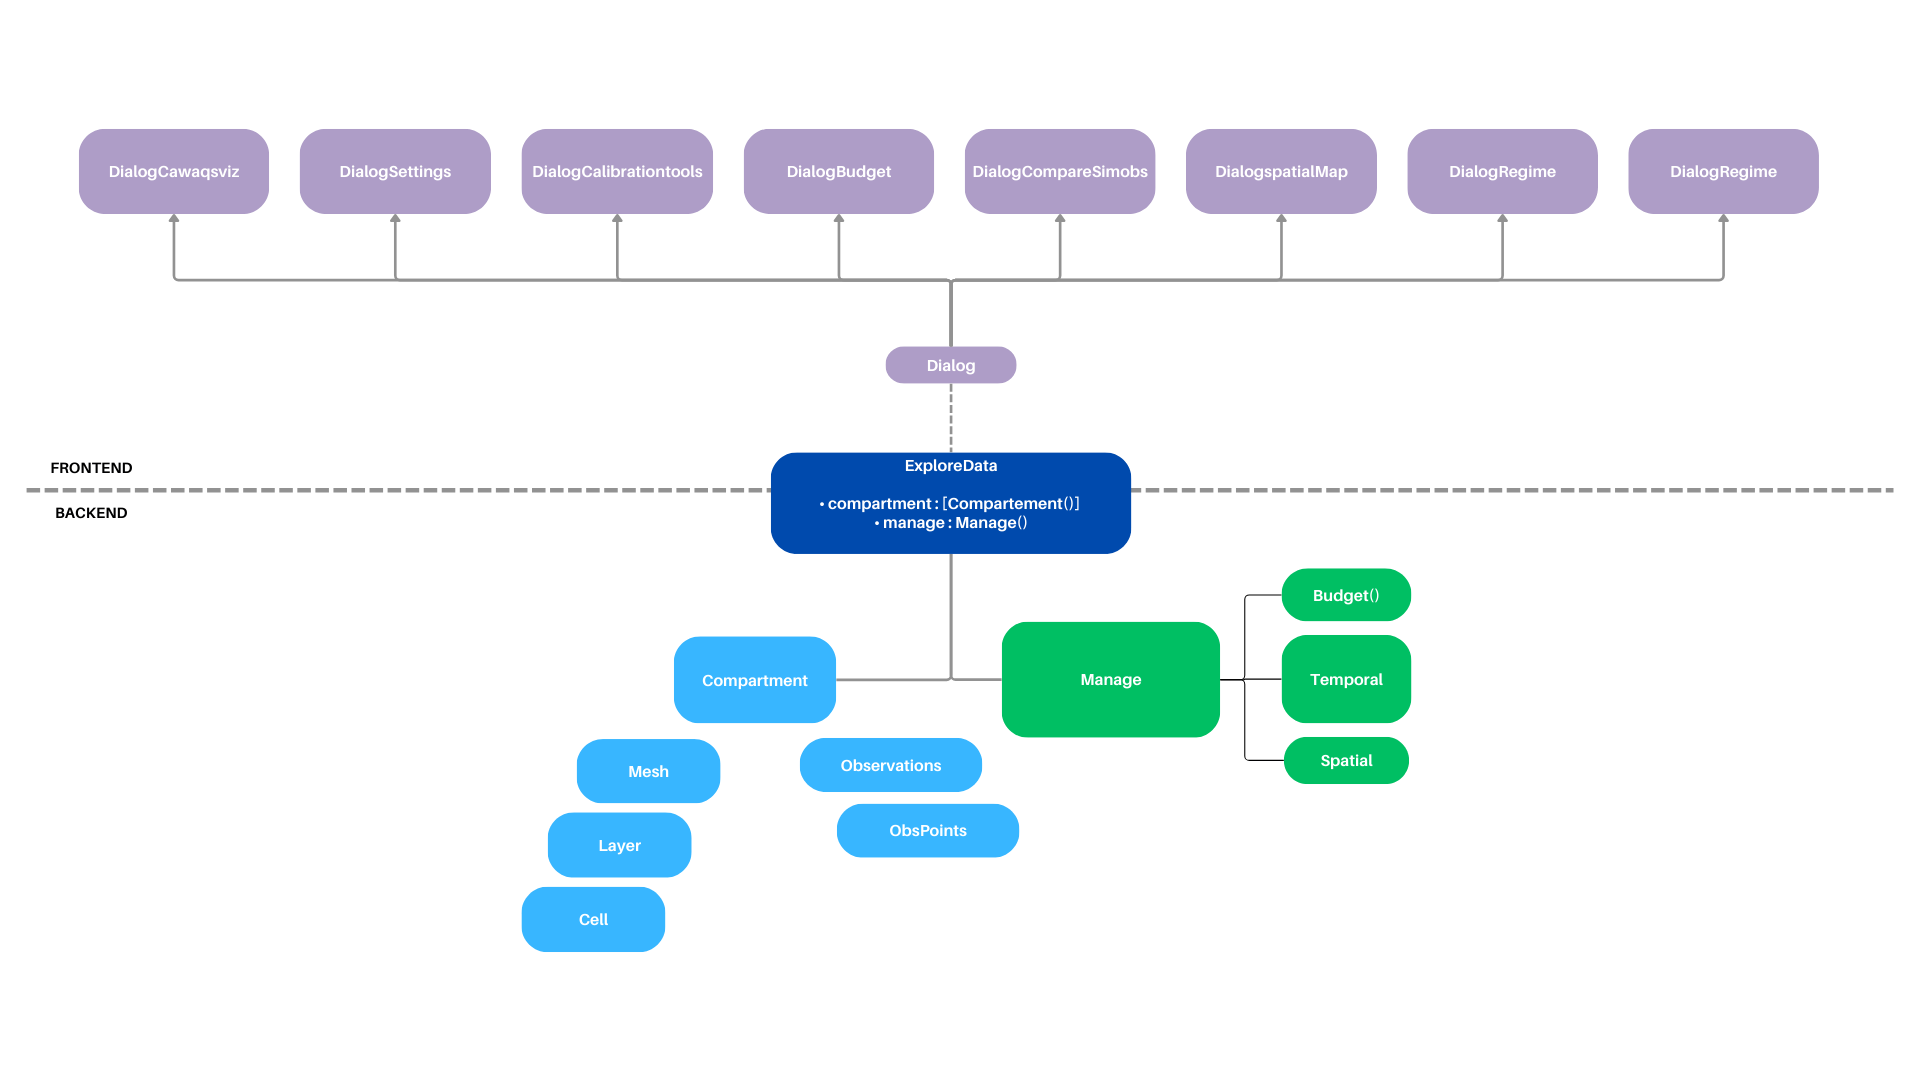
\includegraphics[width=1\linewidth]{
            4_application_scripts/fig/schema_conceptuel_cwv.png
        }
        \caption{Structure du code source du plug-in \cwv.}
        \label{fig-structure_cawaqs_viz}
    \end{figure*}
\end{landscape}

% \section{Détail du back-end}\label{sec-backend}

% ...

% \section{Détail du front-end}\label{sec-frontend}

% ...

% \section{Détail de la passerelle}\label{sec-passerelle}

% ...